\section{Runtime Architecture}

\subsection{Runtime}

\begin{figure}
		\centering
		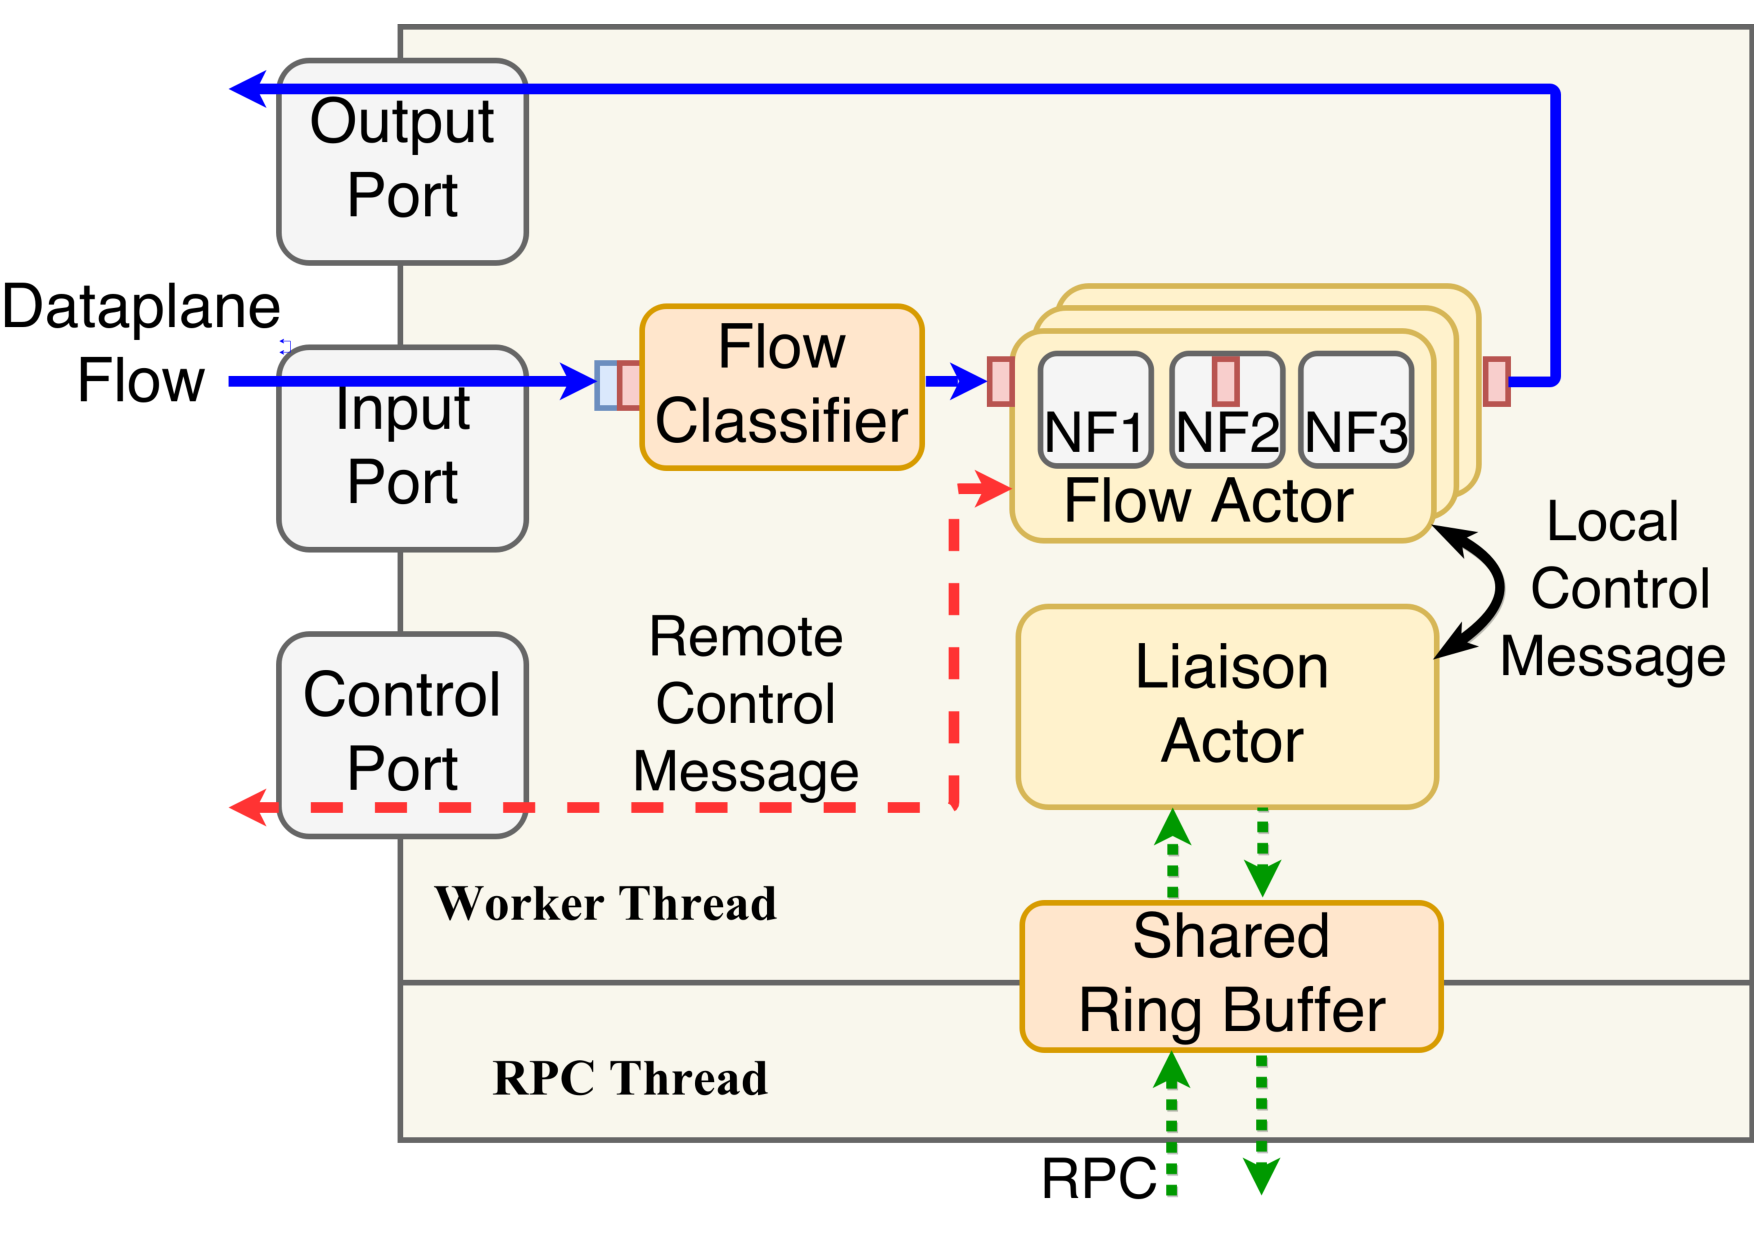
\includegraphics[width=\columnwidth]{figure/new-nfactor-runtime-arch.pdf}

		\caption{The internal architecture of a NFActor runtime system. }
\label{fig:runtime-arch}
\end{figure}

Figure \ref{fig:runtime-arch} demonstrates the internal architecture of a runtime. The runtime serves as a uniform program to run actors. \nfactor~runs each runtime inside a container for fast boot up and assigns each runtime with a global unique ID to ease management. The uniform runtime design increases the scalability of~\nfactor, as \nfactor could be horizontally scaled up by adding more runtimes.

The runtime consists of a single worker thread for actor scheduling, and an RPC thread for receiving RPC requests sent from the controller. The single-worker-thread design guarantees a sequential actor execution order, therefore completely eliminate the need to protect message passing by lock, resulting in a good performance achieved by \nfactor. It is configured with three ports, from which it can send and receive packets. Input packets of the runtime are first sent to a flow classifier, which uses traditional flow-5-tuple (i.e. IP destination address, IP source address, transmission layer protocol, source port and destination port) as the key to classify flows. The flow classifier creates one flow actor for each new flow and forwards all the flow packets to that flow actor.

The runtime is configured with a specific service chain during the boot phase and initializes all the NF modules as specified in the service chain. When a flow actor is created, it loads these modules and uses the flow state allocation method in Table \ref{table:api} to allocates all the flow states and passes input packet along the NF modules in sequence. Besides service chain processing, the flow actor also provides an execution context for distributed flow migration and replication.

There is a coordinator actor who is responsible for executing the RPC requests sent from the controller and coordinate flow actors during flow migration and replication. Flow actor and coordinator actor could directly exchanges local messages, or exchange remote messages through a reliable message passing module \ref{}.

%The runtime is designed as a single-worker-thread architecture to decrease the overhead of flow actors. A high speed NFV system may process millions of packets every second and migrates tens of thousands of flows. At such a high processing rate, message passing protected by shared lock in multi-threaded actor runtime system may incur a huge overhead and hurt the packet throughput.
%The runtime is configured with a specific service chain during the boot phase and initializes all the NF modules as specified in the service chain. When a flow actor is created, it loads these modules and uses the flow state allocation method \ref{table:api} to allocates all the
%To process flows across a service chain, during the initialization phase of the runtime, a service chain specifier is passed in to the runtime. The runtime then loads all the NF modules as indicated in the service chain specifier. When the flow classifier creates a new flow actor, the flow actor also loads these NF modules on the service chain and passes the input packet along the NF modules in sequence.

%The reason that the runtime is designed as a single-worker-thread program is because the multi-worker-thread design may not bring significant performance gain. In our initial prototype implementation, we use LIBCAF \cite{caf} library to construct flow actors. LIBCAF library creates multiple worker threads and schedules flow actors to run on these worker threads. Because LIBCAF completely conceals the internal interfaces of the worker threads, we have to create a dedicated polling thread to poll packet from the input port. Under this design, we find that the maximum throughput of a runtime does not increase when the number of LIBCAF worker thread increases, because the polling thread has always been a bottleneck. Therefore, we abandon the multi-worker-thread design and use a single worker thread to poll packets and schedule flow actors. To our surprise, this architecture turns out to work very well because it allows us to perform aggressive optimization of actor programming model \ref{}. In the mean time, we can still maintain the scalability of the system by launching more runtimes.

\subsection{Virtual Switch}

The virtual switch is a special runtime without service chain, it automatically balances the input traffic among all the runtimes, increasing the scalability of the system. We refer to the flow actor created by the virtual switch as virtual switch actor throughout this paper.

The virtual switch actor selects one of the available runtimes as its destination runtime in a round-robin way when it is created. Round-robin algorithm is used because it imposes the smallest overhead. Whenever the virtual switch actor receives an input packet, it replaces the destination MAC address of the packet to destination runtime's input port MAC address, and modifies the source MAC address of the input packet to virtual switch's output port mac address. it then sends the packet out from the output port.

The architectural consistency of virtual switch and runtime also facilitates flow migration and replication. The flow actor on the destination runtime could analyze the source MAC address of the packet and determine which virtual switch this packet comes from. This enables the flow actor to contact the virtual switch actor during flow migration and replication to change the destination runtime selected by the virtual switch actor \ref{}.

\subsection{Controller and Control RPCs}

%运行时系统暴露了一系列RPC以供controller进行调用。这些rpc可以分为以下几类:控制流管理任务的rpc仅仅

The \nfactor's controller is responsible for monitoring the workload of each runtime and executing dynamic scaling. Due to the use of light-weight and distributed flow actors, the controller only needs to participate in the initiation phase of flow migration and replication. This feature differentiates \nfactor's controller with the controllers in OpenNF \cite{gember2015opennf} and Split/Merge \cite{rajagopalan2013split}, which need to fully coordinate the entire flow migration process. This simplifies the design of the controller and improve the failure resilience, as the controller does not need to maintain complicated states associated with flow migration.

The controller manages \nfactor~using a series of control RPCs exposed by each runtime, which are summarized in Table \ref{table:rpc}. The controller uses PollWorkload RPC to acquire the current workload on a runtime and generates dynamic scaling decision. The controller maintains the configuration of the cluster, which include the mac address of input/output/control port and the ID of all the runtime and virtual switches. The controller notifies the cluster configuration to a runtime using NotifyClusterCfg RPC. The last three RPCs are used to initiate flow migration and replication. After issuing these three calls, migration and replication are automatically executed without further involving with the controller.

\begin{table}[!h]
\centering
\caption{Control RPCs exposed from each runtime.}
\label{table:rpc}
\resizebox{\columnwidth}{!}{
\begin{tabular}{l|l}
Control RPC                                                                                   & Functionality                                                                                                                                              \\ \hline
PollWorkload()                                                                                   & \begin{tabular}[c]{@{}l@{}}Poll the workload information \\ from the runtime.\end{tabular}                                                                 \\ \hline
NotifyClusterCfg(cfg)                                                                         & \begin{tabular}[c]{@{}l@{}}Notify a runtime the current \\ cluster configuration.\end{tabular}                                                             \\ \hline
\begin{tabular}[c]{@{}l@{}}SetMigrationTarget(runtime\_id, \\ migration\_number)\end{tabular} & \begin{tabular}[c]{@{}l@{}}Initiate flow migration. It tells \\ the runtime to migrate \\ migration\_num flows to runtime\\ with runtime\_id.\end{tabular} \\ \hline
SetReplica(runtime\_id)                                                                       & \begin{tabular}[c]{@{}l@{}}Set the runtime with runtime\_id \\ as the replica.\end{tabular}                                                                \\ \hline
Recover(runtime\_id)                                                                          & \begin{tabular}[c]{@{}l@{}}Recover all the flows replicated \\ from runtime with runtime\_id.\end{tabular}                                                 \\ \hline
\end{tabular}
}
\end{table}

\subsection{Resilience}

\subsubsection{Distributed Flow Migration}

\begin{figure}[!h]
\begin{subfigure}[t]{0.33\linewidth}
   \centering
   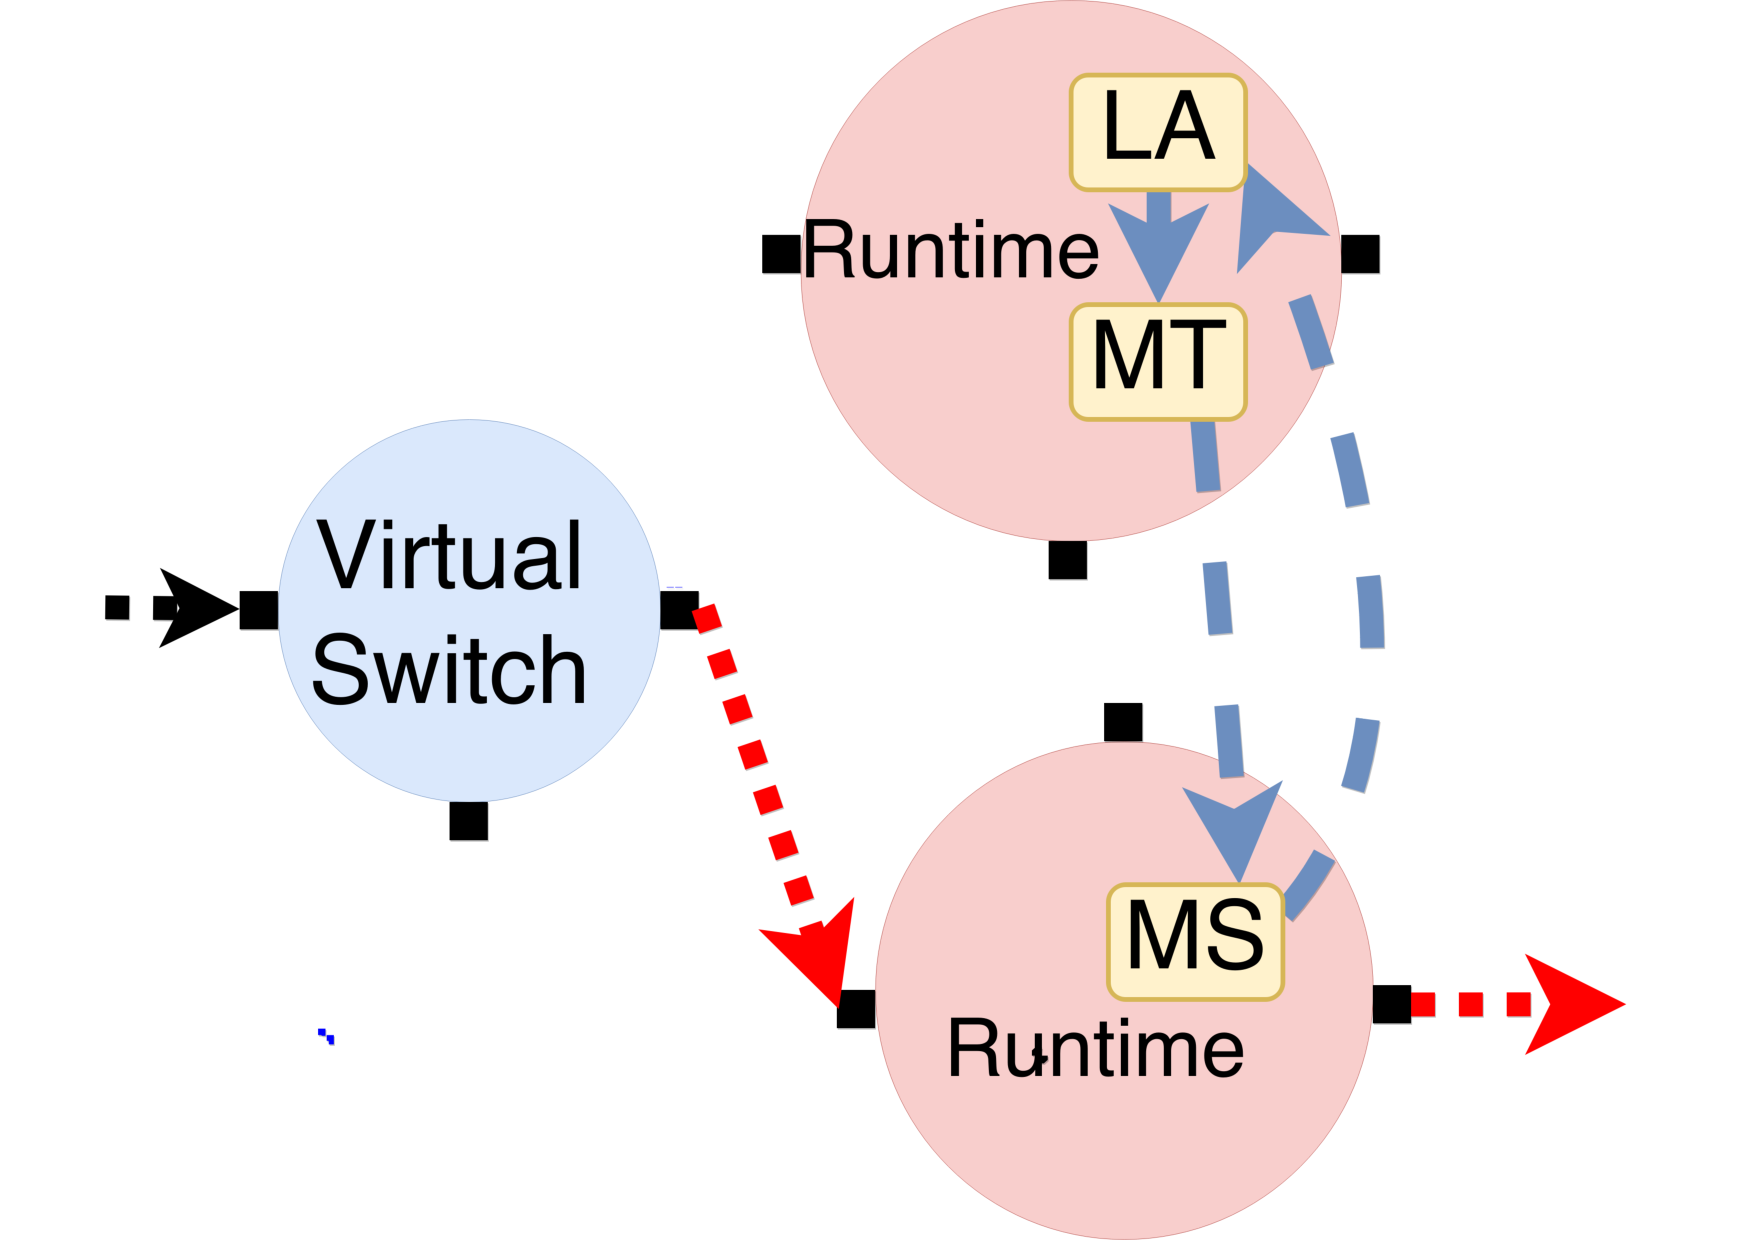
\includegraphics[width=\columnwidth]{figure/nfactor-mig1.pdf}
   \caption{1st req-rep.}\label{fig:mig1}
  \end{subfigure}\hfill
  \begin{subfigure}[t]{0.33\linewidth}
     \centering
     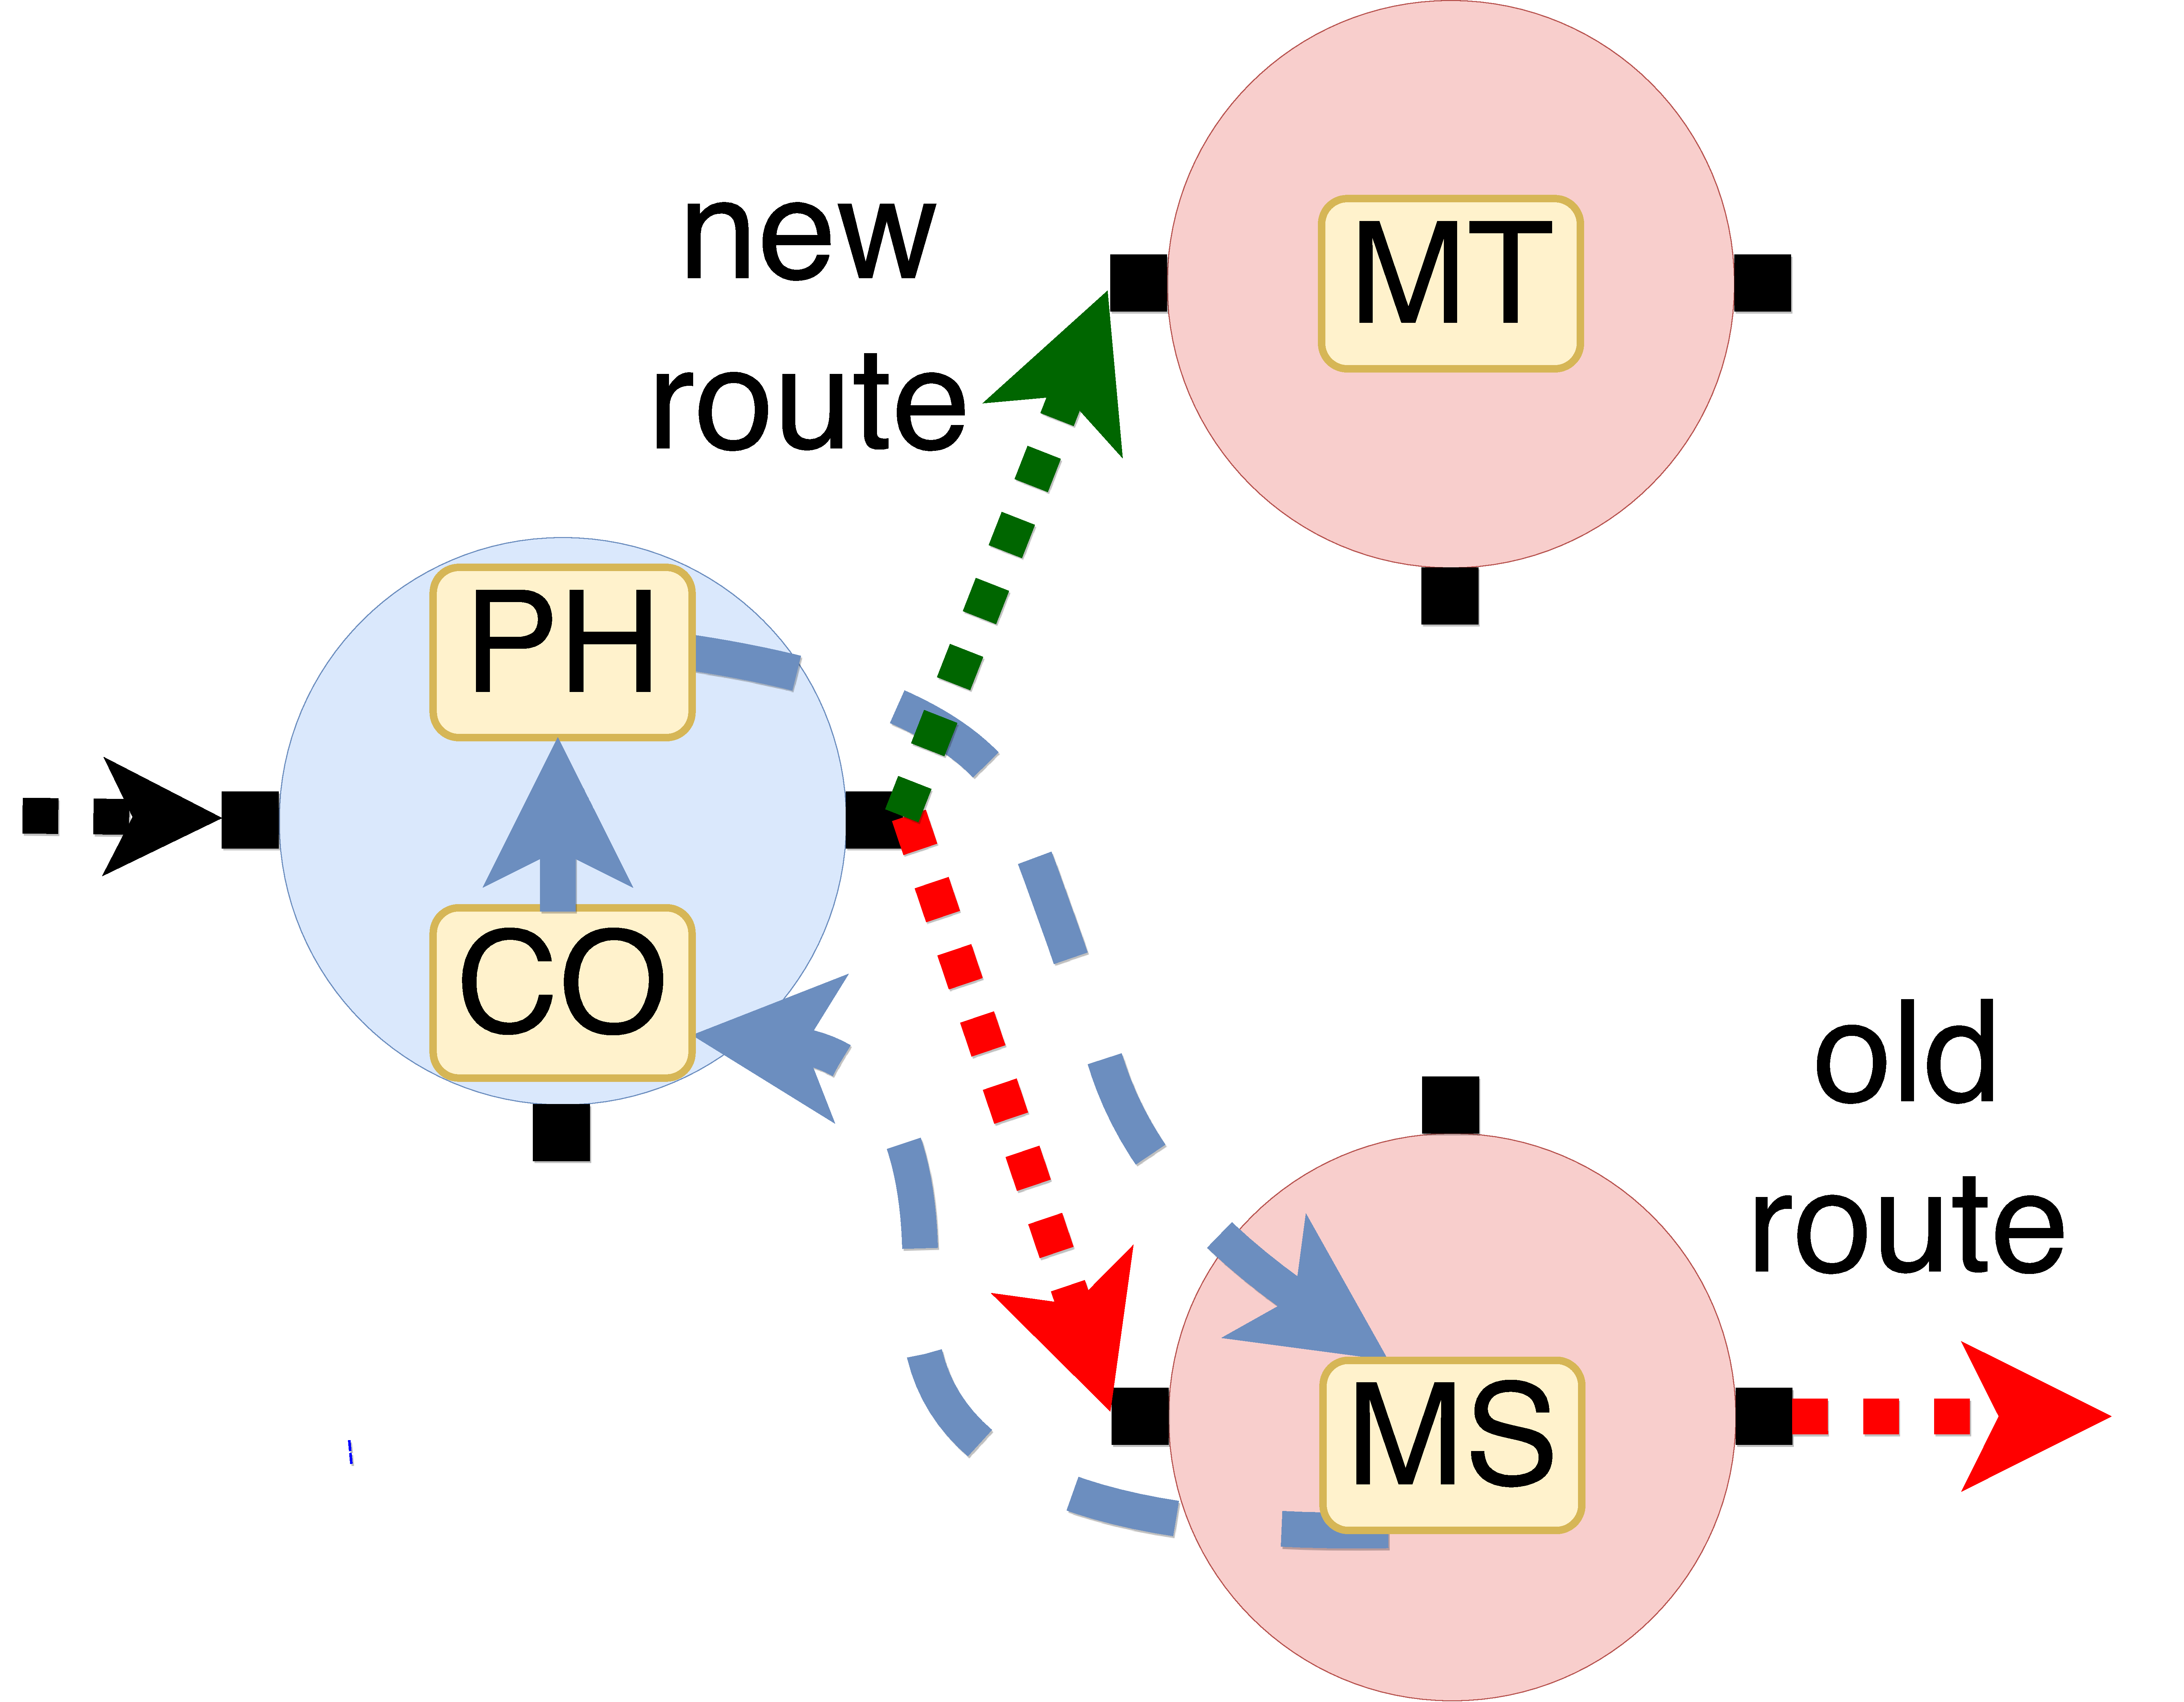
\includegraphics[width=\columnwidth]{figure/nfactor-mig2.pdf}
     \caption{2nd req-rep.}\label{fig:mig2}
    \end{subfigure}\hfill
  \begin{subfigure}[t]{0.33\linewidth}
 \centering
   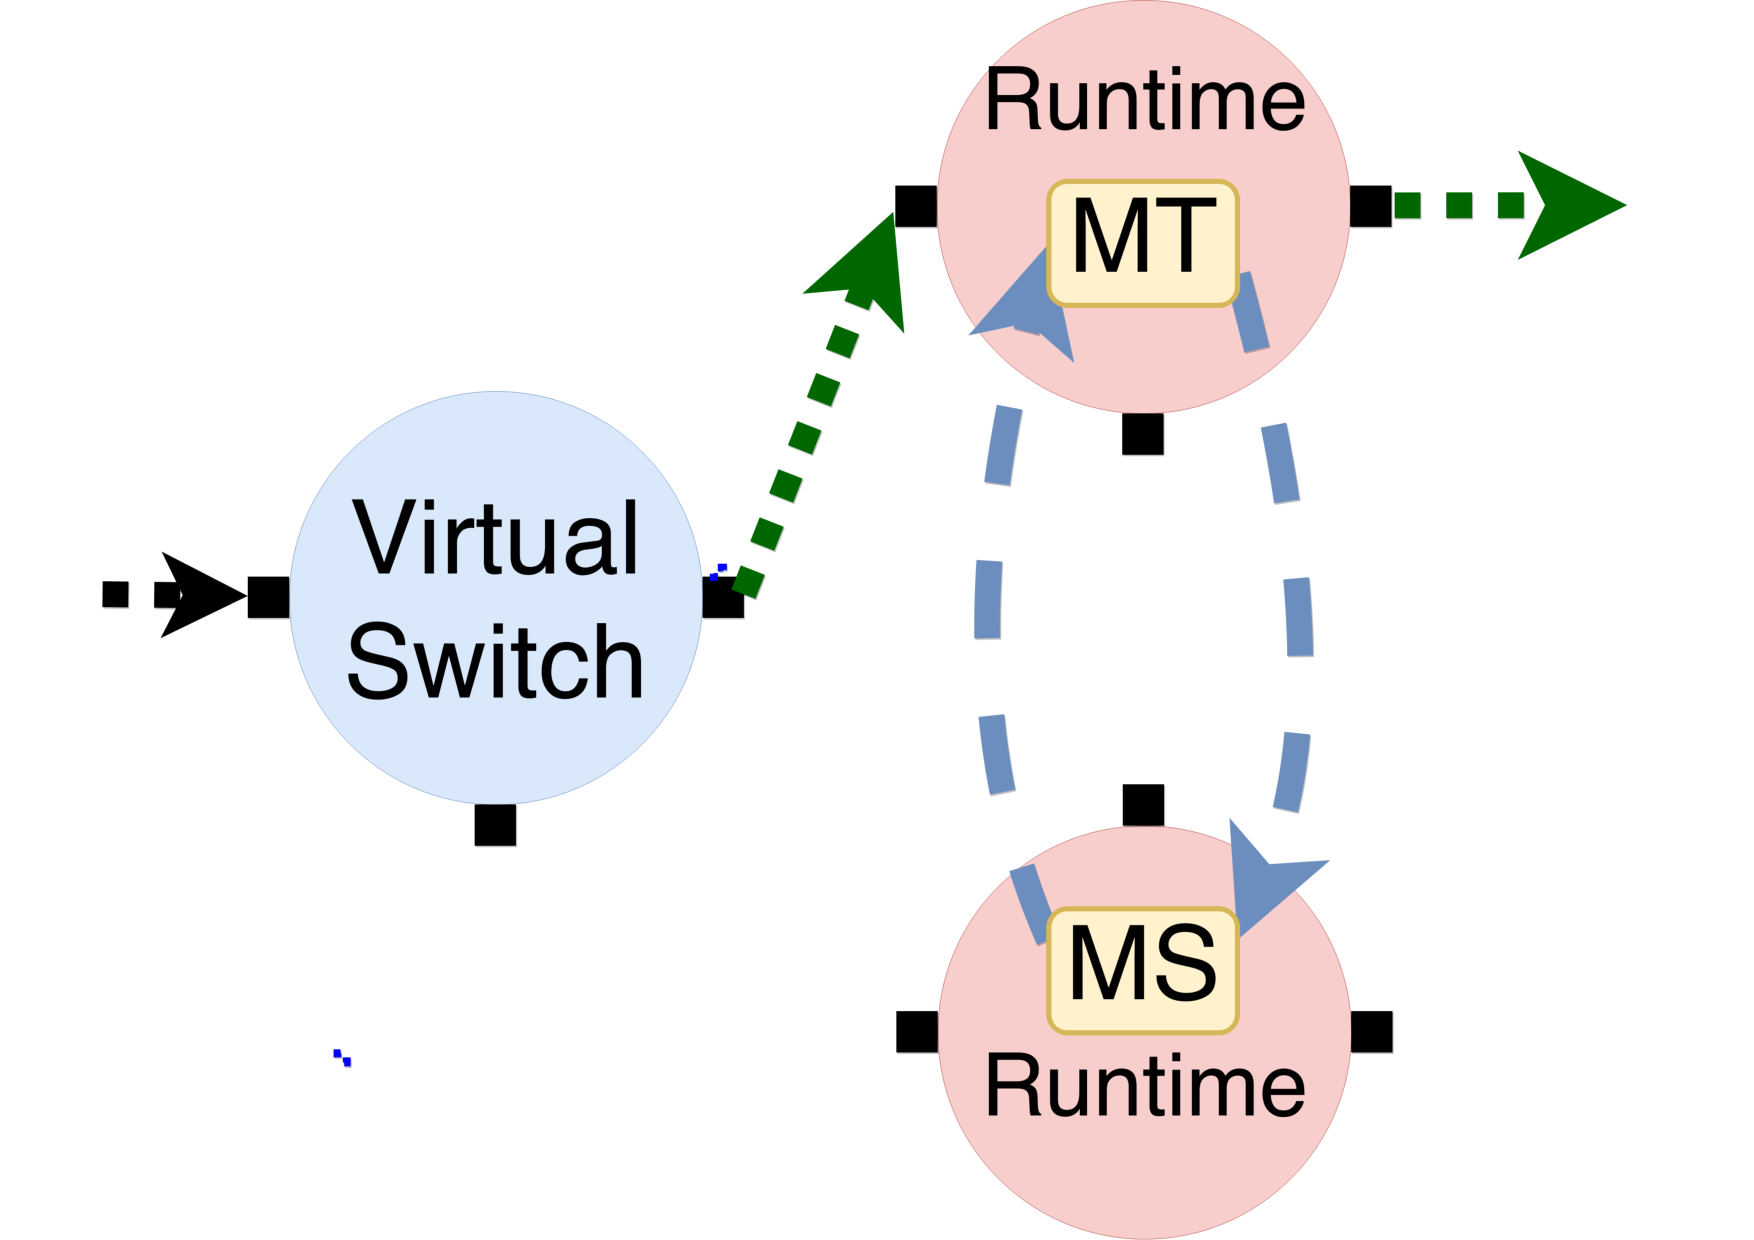
\includegraphics[width=\columnwidth]{figure/nfactor-mig3.pdf}
   \caption{3rd req-rep.}\label{fig:mig3} \end{subfigure}\hfill
 \caption{The flow migration process that migrates migration source actor running on migration source runtime to migration target runtime. (\textbf{MT}: Migration target actor. \textbf{MS}: Migration source actor. \textbf{CO}: Coordinator actor. \textbf{VS}: Virtual switch actor. \textbf{Dotted line}: Dataplane flow packets. \textbf{Dashed line}: Actor messages.)}
\label{fig:mig}
\end{figure}

Figure \ref{fig:mig} shows workflow of \nfactor's flow migration, which involves passing three request-response. Besides being fully distributed, the flow migration also guarantees two properties that (i) except for the migration target side buffer overflow or network packet reordering (which rarely happens in \nfactor), no flow packets are dropped by the flow migration protocol, which we refer to as \textbf{loss-avoidance} property (this is slightly weaker that the loss-free property in OpenNF \cite{gember2015opennf}) and (ii) the same \textbf{order-preserving} property as in OpenNF \cite{gember2015opennf}. There has been a long understanding that providing good properties for flow migration would compromise the performance of flow migration \cite{gember2015opennf}. \nfactor~ breaks this misunderstanding using the novel distributed flow migration.

The details of the three request-responses are summarized below.
\begin{itemize}

\item \textbf{1st req-rep:} The migration source actor sends its flow-5-tuple to the coordinator actor on the migration target runtime. The coordinator actor creates a migration target actor using the flow-5-tuple contained in the request, which returns a response back to the migration source actor. During the execution of the first request-response, migration source actor continues to process packet.

\item \textbf{2nd req-rep:} The current flow actor sends its flow-5-tuple and the ID of the migration target runtime to the coordinator actor on the virtual switch. The coordinator actor uses the flow-5-tuple to find out the virtual switch actor and notifies it to change the destination runtime to migration target runtime. After changing the destination runtime, the virtual switch actor sends a response back to the migration source actor. The migration target actor starts to receive packets after the destination runtime of the virtual switch actor is changed and buffer all the received packets until it receives the third request. In the meantime, the migration source actor keeps processing the input packets until it receives the second response.

\item \textbf{3rd req-rep:} the migration source actor sends its flow state to the migration target actor. After receiving the flow states, the migration target actor saves them, gives a response to the migration source actor and immediately start processing all the buffered packets. The migration source actor exits when it receives the response.

\end{itemize}

\textbf{The Loss-Avoidance Property.} Before the migration target actor receives the third request, it needs to buffer input packets indefinitely, which might lead to a buffer overflow if the third request takes a long time to arrive. \nfactor~ simply drops additional flow packets after buffer overflow because \nfactor~ needs to process packet at a high throughput rate and does not want to grow buffer indifinitely. In \nfactor, a large collective buffer is used to buffer the packets for different migration target actors and the distributed flow migration process is extremely fast, so the buffer overflow rarely happens, even when migrating a huge number of flows. This is demonstrated in the evaluation section \ref{}.

Besides buffer overflow, the only step that might incur potential packet drop is in the third request-response. When the second response is received by the migration source actor, it must immediately send its flow state in the third request to the migration target actor. After sending the third request, there might be pending flow packets continuing to arrive at migration source actor. These pending packets are are sent out by the virtual switch actor before the destination runtime is changed. If this happens, the migration source actor has to discard these pending flow packets because it has already sent out the third request. Continuing to process these packets may generate inconsistent output packets.

If the network doesn't reorder packet, which is a common case because \nfactor~is deployed over a L2 network, \nfactor's flow migration can eliminate the second cause of packet drop by transmitting second response in a network packet over the same network path as the data plane packets that are sent to the migration source actor. Recall that in Figure \ref{fig:runtime-arch}, the remote messages could be sent over input/output port of a runtime. The second response is encapsulated in a raw packet \ref{}, sent by the output port of the virtual switch and received by the input port of the migration source runtime, therefore sharing the same network path as the data plane packets that are sent to the migration source actor.

Because the second response are sent after the destination runtime of the virtual switch actor is changed and share the same network path as the data plane packets that are sent to the migration source actor, it also becomes a strong indication that no more input packets will be sent to the migration source actor. This is verified in our evaluation \ref{}.

\textbf{Order-preserving Property.} Since the second request-response eliminate the packet drop if the network doesn't reorder packets, flow packets could always be processed in the order that they are sent out from the virtual switch. The order-preserving property is therefore guaranteed.

\textbf{Error Handling.} The three request-responses may not always be successfully executed. In case of request timeout, the migration source actor is responsible for restoring the destination runtime of the virtual switch actor (if it is changed) and resumes normal packet processing. The migration target actor is automatically deleted after a timeout.

\subsubsection{Scalable Flow Replication}

\begin{figure}[!h]
\begin{subfigure}[t]{0.49\linewidth}
   \centering
   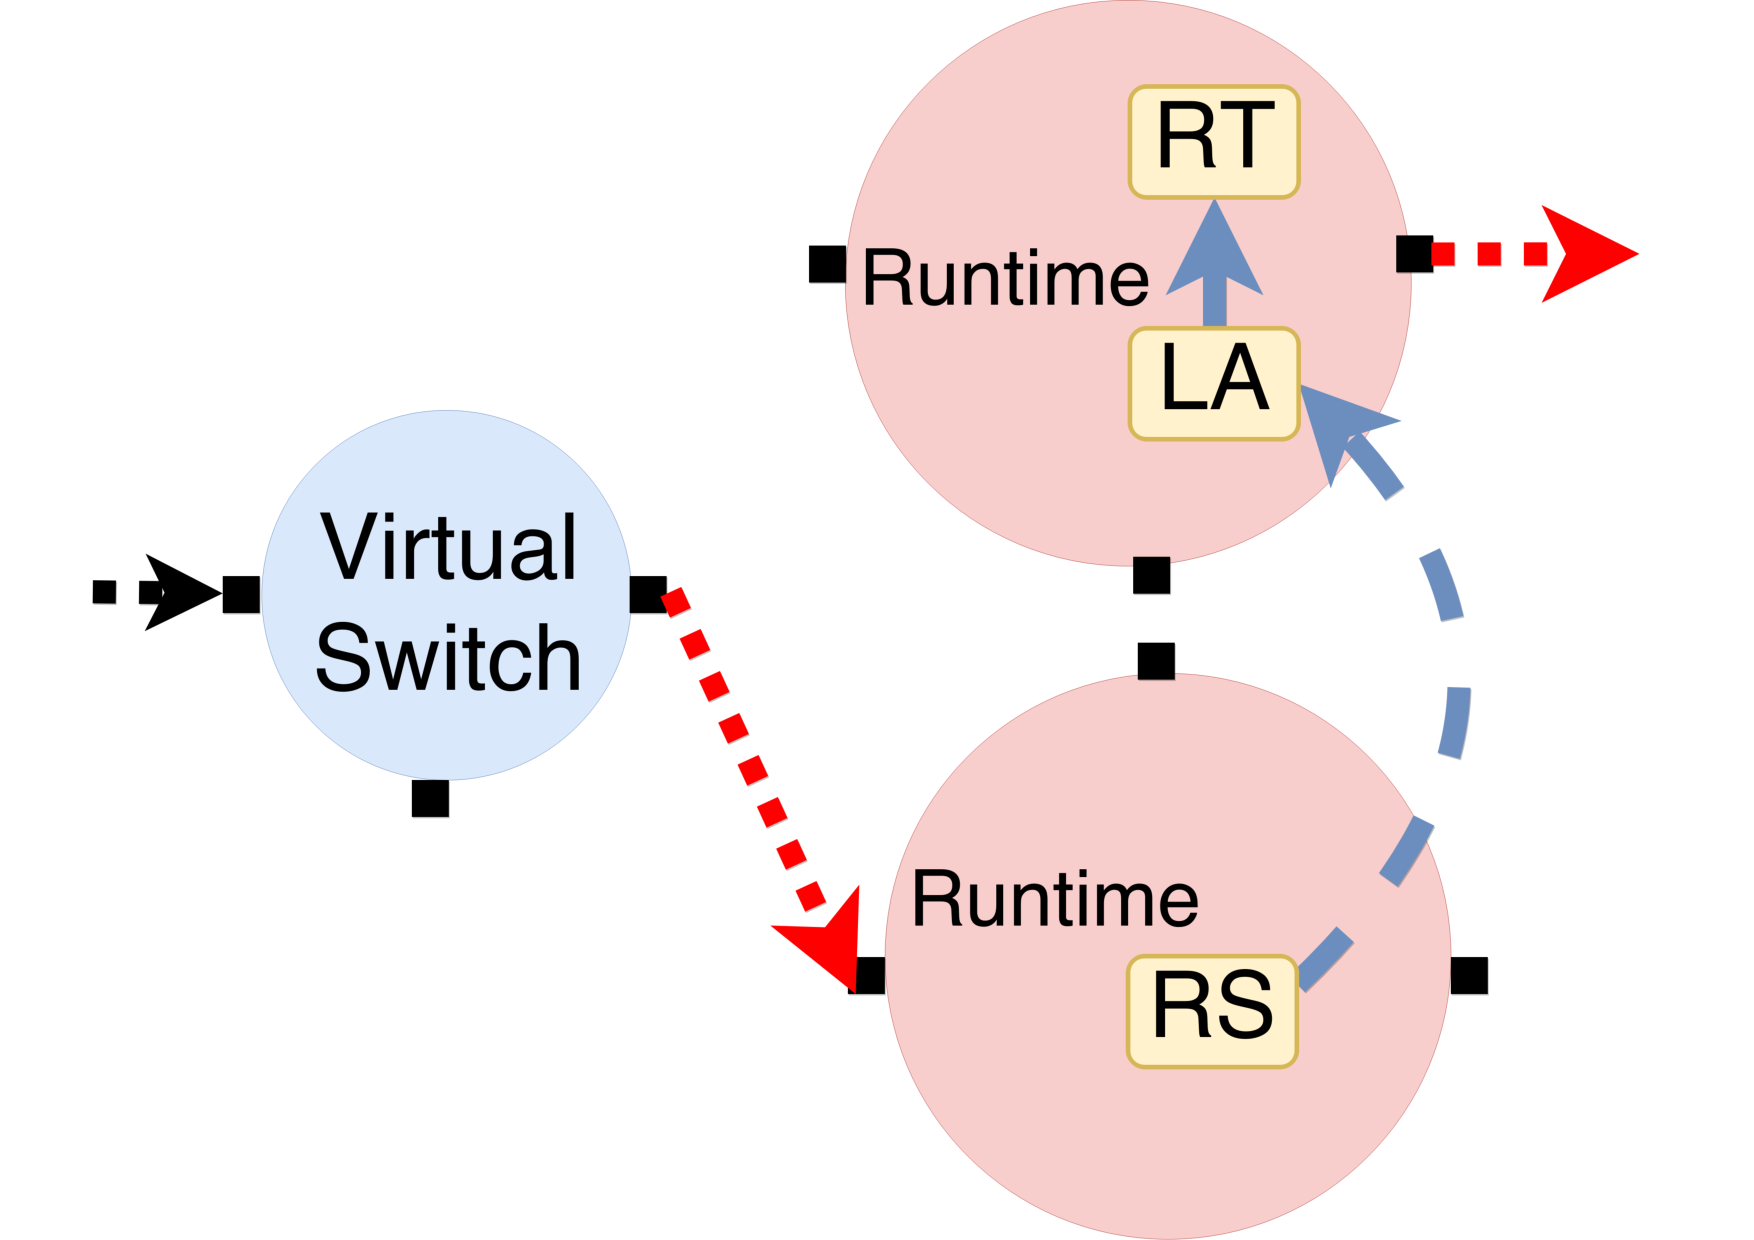
\includegraphics[width=0.66\columnwidth]{figure/nfactor-replication.pdf}
   \caption{Flow replication.}\label{fig:rep}
  \end{subfigure}
  \begin{subfigure}[t]{0.49\linewidth}
     \centering
     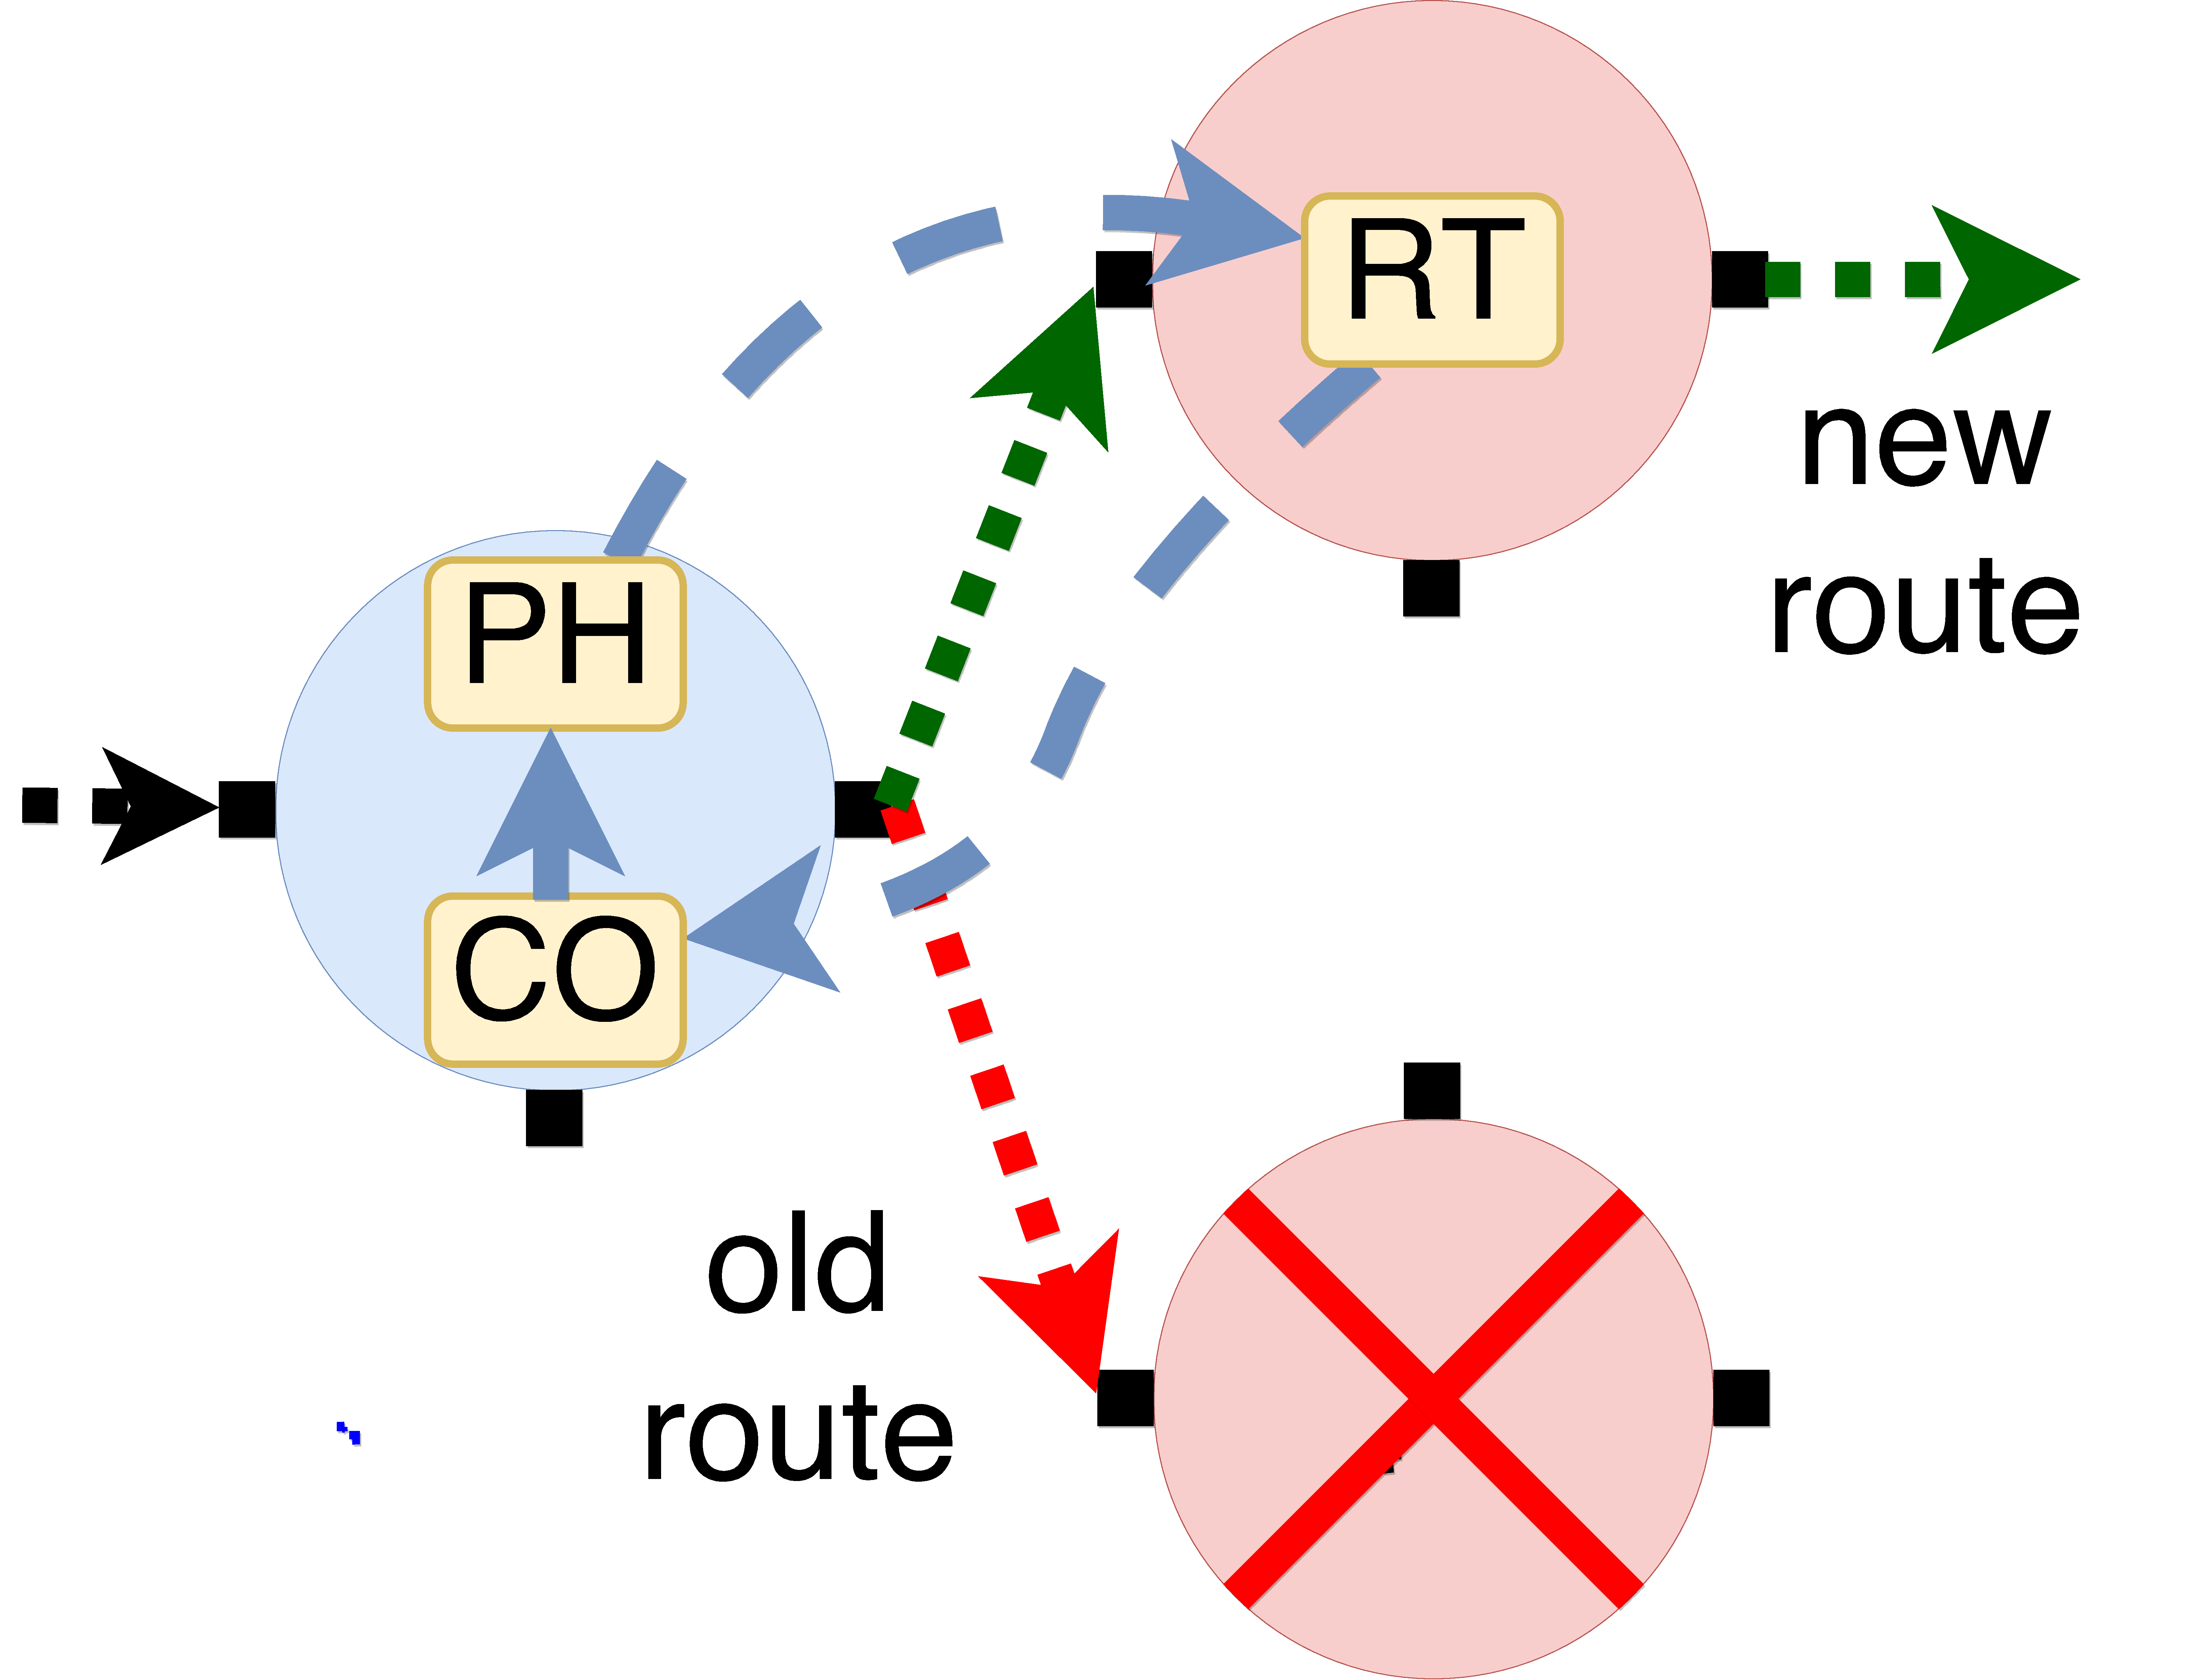
\includegraphics[width=0.66\columnwidth]{figure/nfactor-recover.pdf}
     \caption{Flow recover. The original runtime has failed.}\label{fig:recover}
    \end{subfigure}
 \caption{Flow replication that replicates the original actor running on the original runtime to replica runtime. (\textbf{RT}: Replication target actor. \textbf{RS}: Replication source actor. \textbf{CO}: Coordinator actor. \textbf{VS}: Virtual switch actor. \textbf{Dotted line}: Dataplane flow packets. \textbf{Dashed line}: Actor messages.)}
\label{fig:flow-rep}
\end{figure}

The biggest difference of the \nfactor's replication method and existing works such as \cite{sherry2015rollback} is that NFActor framework replicates individual flow, not NF. This replication strategy is transparent to the NF modules and improves the scalability and resource utilization rate of \nfactor. as flows could be directly replicated on another runtime, without the need for a dedicated backup server. In the mean time, this fine grained replication strategy provides a the same output-commit property as indicated in \cite{sherry2015rollback} with a desirable replication throughput and fast recovery time.

The detailed flow replication process is shown in figure \ref{fig:flow-rep}. When a flow actor is created, it acquires its replica runtime by querying a round-robin list. If the flow actor has a valid replica runtime, whenever it finishes processing the packet, it sends a remote message, containing the current flow state and the packet, to the coordinator actor on the replication target runtime. The coordinator actor on the replication target runtime creates a replica flow actor using the same flow-5-tuple as the original flow actor to handle all the replication messages. The replica flow actor saves the flow state and sends the packet out from the output port of the replica runtime. Similar with \cite{sherry2015rollback}, the receiver on the side of the output port of the replica runtime can only observe an output packet when the flow state has been replicated.

When a runtime fails, the controller sends recovery RPC requests \ref{} to all the replica runtime of the failed runtime. This RPC enables replica flow actor to send a request to the virtual switch actor, asking it to change the destination runtime to the replica runtime. When the response is received by the replica flow actor, the original flow is successfully restored on the replica runtime.

\subsection{Design Discussion}

A runtime in NFActor framework is configured with a single service chain. Each flow is handled by a unique actor, which carries out all the processing on the configured service chain. Alternative design options do exist, however, they may not fully achieve our design goal to achieve low overhead and high scalability.

There are two alternatives to the one-flow-one-actor design. First of all, using a single flow actor to process multiple flows compromise the efficiency of flow migration protocol, especially when multiple flows come from different virtual switch actors. Under this situation, the flow actor must synchronize the responses sent from different virtual switch actors, therefore decreasing the performance of migration. Secondly, chaining several flow actors together to process the same flow imposes unnecessary overhead for flow processing. Therefore, the one-flow-one-actor design achieves a sweet point in minimizing the actor processing overhead and improving the efficiency of flow migration protocol design.

The alternative design to one-runtime-one-service-chain is to dynamically configure multiple service chains on a single runtime. Then due to the one-flow-one-actor design, we need to do an additional service chain selection, based on some pre-defined rules. This adds additional overhead to the flow actor processing and increases the complexity when managing the NFActor cluster, because the controller must populates the service chain rule dynamically to each runtime. With the one-runtime-on-service-chain design, if another service chain is needed, the system administrator could launch a new NFActor cluster and configure a different service chain to use.
